\section{Testy}
	\label{testy}
    Technologie internetowe rozwijają się w zastraszającym tempie, co za tym idzie, wymagania klientów również. Wiele firm kładzie duży nacisk na testowanie swoich aplikacji.

  	Programiści często wychodzą z założenia, że ,,najpierw kod, później testy". Ma to oczywiście swoje wady i zalety. Zaletą niewątpliwie jest czas realizacji. Wynika to z tego, że w pierwszej kolejności pisze się daną funkcjonalność i nie zastanawia się nad tym jak napisać do niej test. Po skończeniu przychodzi czas na napisanie testów do niej. Wygląda to mniej więcej tak, że pisze się jeden lub dwa testy, które sprawdzą czy funkcjonalność w ogóle działa i dodatkowo kilka skrajnych przypadków w których może się wysypać. Doprowadza to do tego, że cały kod jest pokryty testami w bardzo małym stopniu, więc tak naprawdę w każdej chwili może zajść sytuacja, w której przestanie to działać tak jak powinno. Niestety w takim przypadku tracimy cenne godziny na szukanie błędu i jego eliminację.

  	My w swojej pracy przyjęliśmy zupełnie inne podejście, mianowicie ,,najpierw testy, później kod". Owszem, czas pisania znacznie się wydłuża, ale kod jest w dużo większym stopniu pokryty testami, dzięki czemu oszczędzamy sporo godzin przy diagnozie danego błędu. Kolejną zaletą takiego podejścia jest to, że napisany w ten sposób kod robi dokładnie to czego oczekujemy. Piszemy test i spełniamy go w najprostszy możliwy sposób. W ten sposób na jedną metodę przypada kilka lub nawet kilkanaście testów, ale kiedy któryś z nich się nie spełni, wiadomo od razu gdzie szukać przyczyny.

  \subsection{Techniki tworzenia oprogramowania}
    \begin{itemize}
      \item Test Driven Development\cite{tdd} \\
        Technika tworzenia oprogramowania, sterowana przez testy. Polega na wielokrotnym powtarzaniu 3 kroków do momentu ukończenia funkcjonalności:
        \begin{enumerate}
          \item Napisanie możliwie najprostszego testu jednostkowego, który ma sprawdzać kod pisany w kroku 2.
          \item Implementacja kodu. Kod powinien być napisany w taki sposób, aby spełnić założenia testu, nic ponad to. Test powinien zakończyć się sukcesem i nie naruszać pozostałych testów
          \item Refaktoryzacja. Doprowadznie kodu do stanu, w którym spełnia przyjęte normy i standardy prostego oraz czytelnego kodu\cite{scs}.
        \end{enumerate}

        Postępowanie według tego schematu, zmusza programistę do wcześniejszego przemyślenia funkcjonalności, którą ma napisać.

        Wady:
        \begin{itemize}
          \item Wydłuża się czas pisania aplikacji, zwłaszcza w początkowej fazie wdrażania tej techniki, lecz wraz z ilością napisanych testów jednostkowych, rośnie wydajność ich pisania.
          \item Wraz z rozrostem aplikacji rośnie również ilość testów. Dopóki funkcjonalności są dopisywane, problem nie istnieje. Problem pojawia się w momencie zmian jakiejkolwiek z nich. Trzeba się przygotować na modyfikacje istniejących do niej testów.
        \end{itemize}

        Zalety:
        \begin{itemize}
          \item Główną zaletą tej metodologii jest szybkość diagnozy błędu. Dzięki temu oszczędzamy mnóstwo czasu, który w sytuacji bez testów musielibyśmy poświęcić na dogłębne analizowanie kodu, zastanawianie się co robi dana metoda. Wiadomo ile czasu zajmuje naprawienie kodu napisanego godzine wcześniej, a co dopiero napisanego tydzień czy miesiąc temu.
          \item Jeżeli testy są pisane w odpowiedni sposób, mogą stanowić bardzo dobrą dokumentację. Wystarczy zajrzeć do testu i widać czego programista oczekiwał od konkretnej metody.
          \item Bardziej przemyślany kod. W pierszej kolejności musimy się zastanowić co dana funkcjonalność ma robić, żeby móc od niej to wyegzekować.
        \end{itemize}

        \begin{figure}
          \centering
          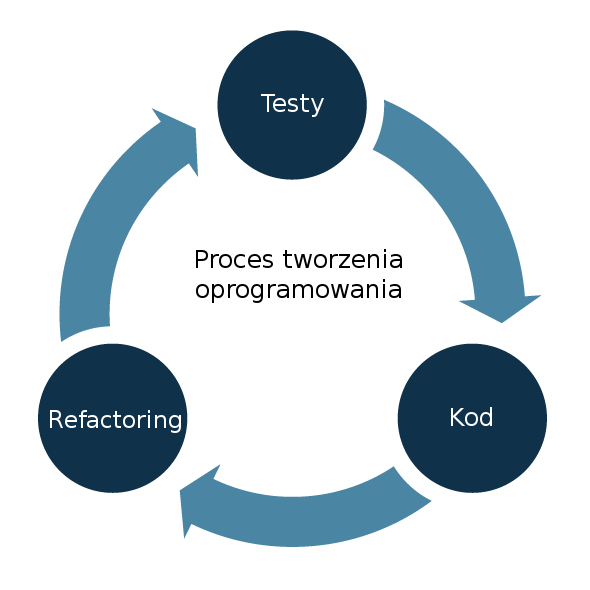
\includegraphics[scale=0.47]{images/test_cycle.png}
          \caption{Schemat postępowania w TDD}
        \end{figure}

      \newpage
      \item BDD \\
      Behaviour Driven Development
    \end{itemize}

	\newpage
  \subsection{Testy integracyjne}
  \subsection{Testy jednostkowe}
